\chapter[Metodologia]{Metodologia}


Este capítulo foi elaborado para melhorar o entendimento das atividades
 realizadas para a produção deste trabalho. O fluxo da Figura 
\ref{fig:fases_metodologia} define estas atividades.

\begin{figure}[h]
    \centering
        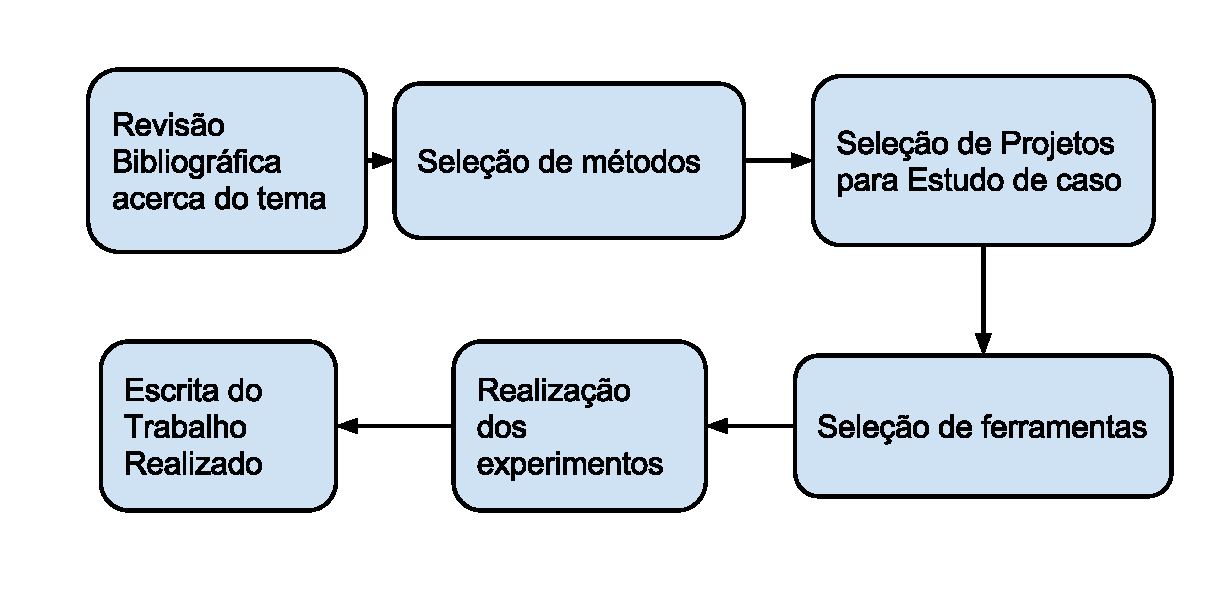
\includegraphics[keepaspectratio=true,scale=0.7]{figuras/fases_metodologia.eps}
    \caption{Fluxo de Atividades para a resolução destes trabalho}
    \label{fig:fases_metodologia}
\end{figure}


\section{Revisão Bibliográfica}

A revisão bibliográfica foi a primeira atividade realizada para a construção
 deste trabalho. Foi feito um estudo e levantamento de métodos, técnicas e
 ferramentas que podem auxiliar o desenvolvimento deste trabalho, além de
 elucidar a viabilidade da realização do mesmo. Esta revisão foi utilizada
 como referência para a  escrita da fundamentação teórica.

\section{Seleção de Métodos}

Para seleção de métodos foi realizada uma priorização dos métodos, técnicas e
 ferramentas encontradas durante a revisão bibliográfica. A priorização levou
 em conta o esforço da implementação/execução dos métodos, o tempo para a
 montagem de cada caso e o recurso computacional necessário para a criação
 destes.

Os métodos selecionados foram:

\begin{itemize}
	\item \textit{Include Guards}, descrito na Seção
 \ref{include_guards_section};
	\item \textit{Forward Declaration}, descrito na Seção
 \ref{forward_declaration_section};
	\item Makefile, descrito na Seção
 \ref{Makefile_section};
	\item Otimização de baixo nível descrito na Seção
 \ref{Otimizacao_de_baixo_nivel};
	\item \textit{Pimpl Idiom} descrito na Seção
 \ref{Pimpl_Idiom};
	\item As ferramentas de otimização descritas na Seção
 \ref{ferramentas_de_otimizacao};
\end{itemize}

\section{Seleção de Projetos}

\subsection{Método de Seleção}

Para a seleção dos projetos foram analisadas 3 plataformas de controle de informação
de software livre: \textit{Openhub}, \textit{Github}, \textit{Gitlab}.

\textit{Openhub}, conhecido como Black Duck Open Hubi, é uma plataforma que busca dados através
 dos sistemas de versionamento (tais como CVS, Git, Subversion, Bazaar e Mercurial),
 exibindo estatísticas sobre o histórico de um projeto e métricas do software.
 Esta plataforma não foi selecionada devido a possuir um sistema de busca baseada em \textit{tags},
 o que dificultava encontrar projetos específicos, pois o desenvolvedor que deve prover
 informações do projeto, e em alguns casos estas informações estão incoerentes e ou
 redundantes. Além disso não havia sistema de busca avançado.

\textit{Gitlab} é uma plataforma de gerenciamento de software que permite os
 desenvolvedores criarem uma instância própria da ferramenta para o armazenamento
 de um projeto de software em uma infraestrutura própria. Esta ferramenta foi
 descartada pois também possui sistema de \textit{tags} para localizar projetos de uma linguagem,
não permite selecionar múltiplas tags e não possui filtro de pesquisa avançada.

\textit{Github} é uma plataforma de gerenciamento de projetos de software que
utiliza o sistema de versionamento \textit{git}. Esta plataforma foi selecionada devido a
 possibilidade de fazer pesquisa avançada utilizando \textit{tags}, selecionar quantidade de \textit{forks},
 linguagem principal do projeto, conteúdo de texto dentro da descrição de um projeto e
 quantidade de estrelas dadas para um projeto.


A pesquisa avançada foi realizada no dia 27 de agosto de 2015, utilizando os seguintes critérios:

\begin{itemize}
    \item \textbf{Busca por palavra chave nas informações dos projetos}
        \begin{enumerate}[label=\roman* )]
        \item \textbf{mac os} - esta palavra foi selecionada para encontrar projetos
 que poderiam ser compilados em um sistema operacional da Apple. Este sistema tem
 como padrão o compilador clang e gcc/g++ como \textit{front-end}  e como \textit{back-end} possui o LLVM.
        \item \textbf{windows} - esta palavra foi selecionada para encontrar 
 que possui compatibilidade com suporte ao compiladores gcc/g++.
\footnote{Para instalar um compilador é necessário utilizar uma ferramenta de criação de ambiente de desenvolvimento como \textit{cygwin}, \textit{mingw}, \textit{Visual Studio}, entre outros.}
        \item \textbf{linux} - esta palavra foi selecionada para encontrar projetos
 que seja possível compilar em um sistema operacional Linux. Este vem por padrão com
 o compilador g++/gcc.
        \end{enumerate}
    \item \textbf{Linguagem}
        \begin{enumerate}[label=\roman* )]
            \item \textbf{language: C++} - diretriz utilizada para restringir a busca de 
projetos que utilizam a linguagem C++ na maior parte de seu código.
        \end{enumerate}
    \item \textbf{Quantidade de Forks}
        \begin{enumerate}[label=\roman* )]
            \item \textbf{ > 10 forks} - diretriz para selecionar projetos com
 mais de 10 \textit{forks}.
        \end{enumerate}
    \item \textbf{Quantidade de Estrelas}
        \begin{enumerate}[label=\roman* )]
            \item \textbf{ < 10000 stars } - diretriz utilizada para projetos com menos
 de 10 mil estrelas, indicando que pelo menos 10 mil pessoas gostaram do projeto e este
é fortemente utilizado. 
        \end{enumerate}
\end{itemize}

Após esta pesquisa avançada foram selecionado os 5 primeiros projetos.

\begin{lstlisting}[language=python, caption={Busca avançada github },
                  label=busca_avanacada_github]
     linux windows mac os  language:C++  stars:<10 00 forks: > 10
\end{lstlisting}


\begin{figure}[h]
    \centering
        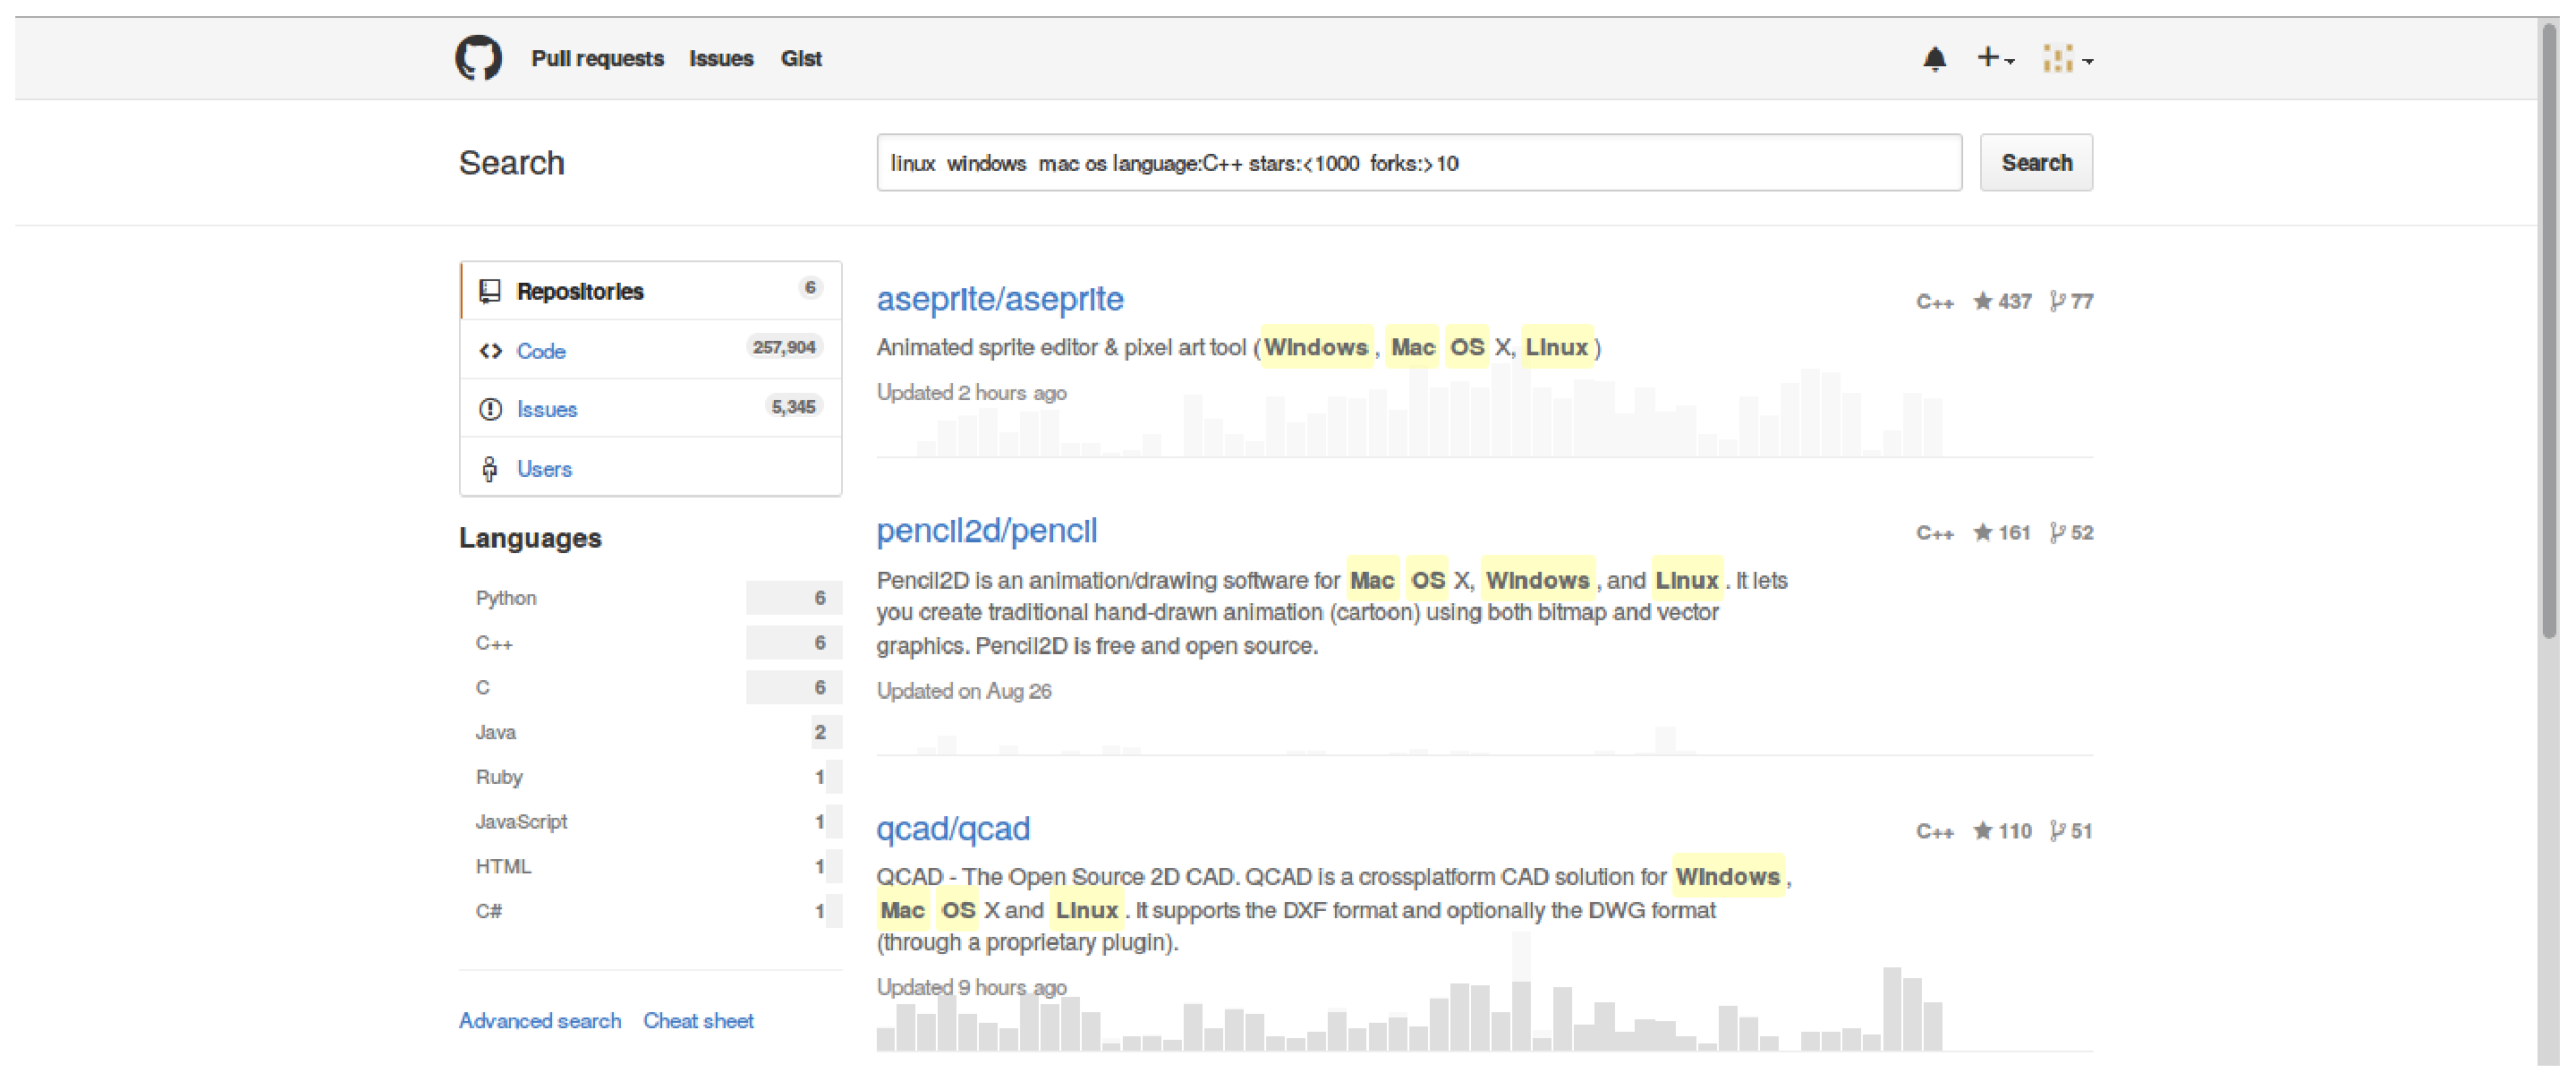
\includegraphics[scale=0.40]{figuras/github_search_1.eps}
    \caption{Pesquisa avançada Github parte 1}
    \label{pesquisa_github}
\end{figure}
\begin{figure}[h]
    \centering
        
\includegraphics[scale=0.40]{figuras/github_search_2.eps}
    \caption{Pesquisa avançada Github parte 2}
    \label{pesquisa_github}
\end{figure}


\begin{table}[h]
\centering
\tiny
\caption{Projetos Selecionados}
\label{projetos_selecionados}
\begin{tabular}{llllll}
\textbf{Projeto} & \textbf{Linguagem} & \textbf{Estrelas} & \textbf{Forks} & \textbf{Porcentagem em C++} & \textbf{Gerador de Makefile}\\ \toprule
Aseprite & C++ & 437  & 77  & 62,1\% & CMake \\ \midrule 
Pencil & C++ &  161 & 22  & 54,6\%   & QMake \\ \midrule
Qcad & C++ & 110 & 51 & 80,8\%       & QMake \\ \midrule 
Sudoku & C++ &  44  & 24 & 94,9\%    & Qmake \\ \midrule
iRecoveryplusplus & C++ & 17 & 11 & 84,7\% & -  \\ \bottomrule
\end{tabular} 
\end{table}


\subsection{Sobre os Projetos}

\begin{itemize}
    \item \textbf{Asepriter}
 \footnote{\url{http://www.aseprite.org/}} é uma ferramenta para criação de \textit{sprites},
 compostas por camadas e quadros, com suporte a RGBA, paleta de 256 cores e escala de cinza.
 Permite visualizar a animação em tempo real e contém ferramentas para preencher contornos
 e polígonos. Esta ferramenta e open source e livre, e pode ser encontrada no \textit{Github}
 \footnote{\url{https://github.com/aseprite/aseprite}} ou no site da ferramenta
 \footnote{\url{http://www.aseprite.org/}}.

    \begin{figure}[h]
        \centering
            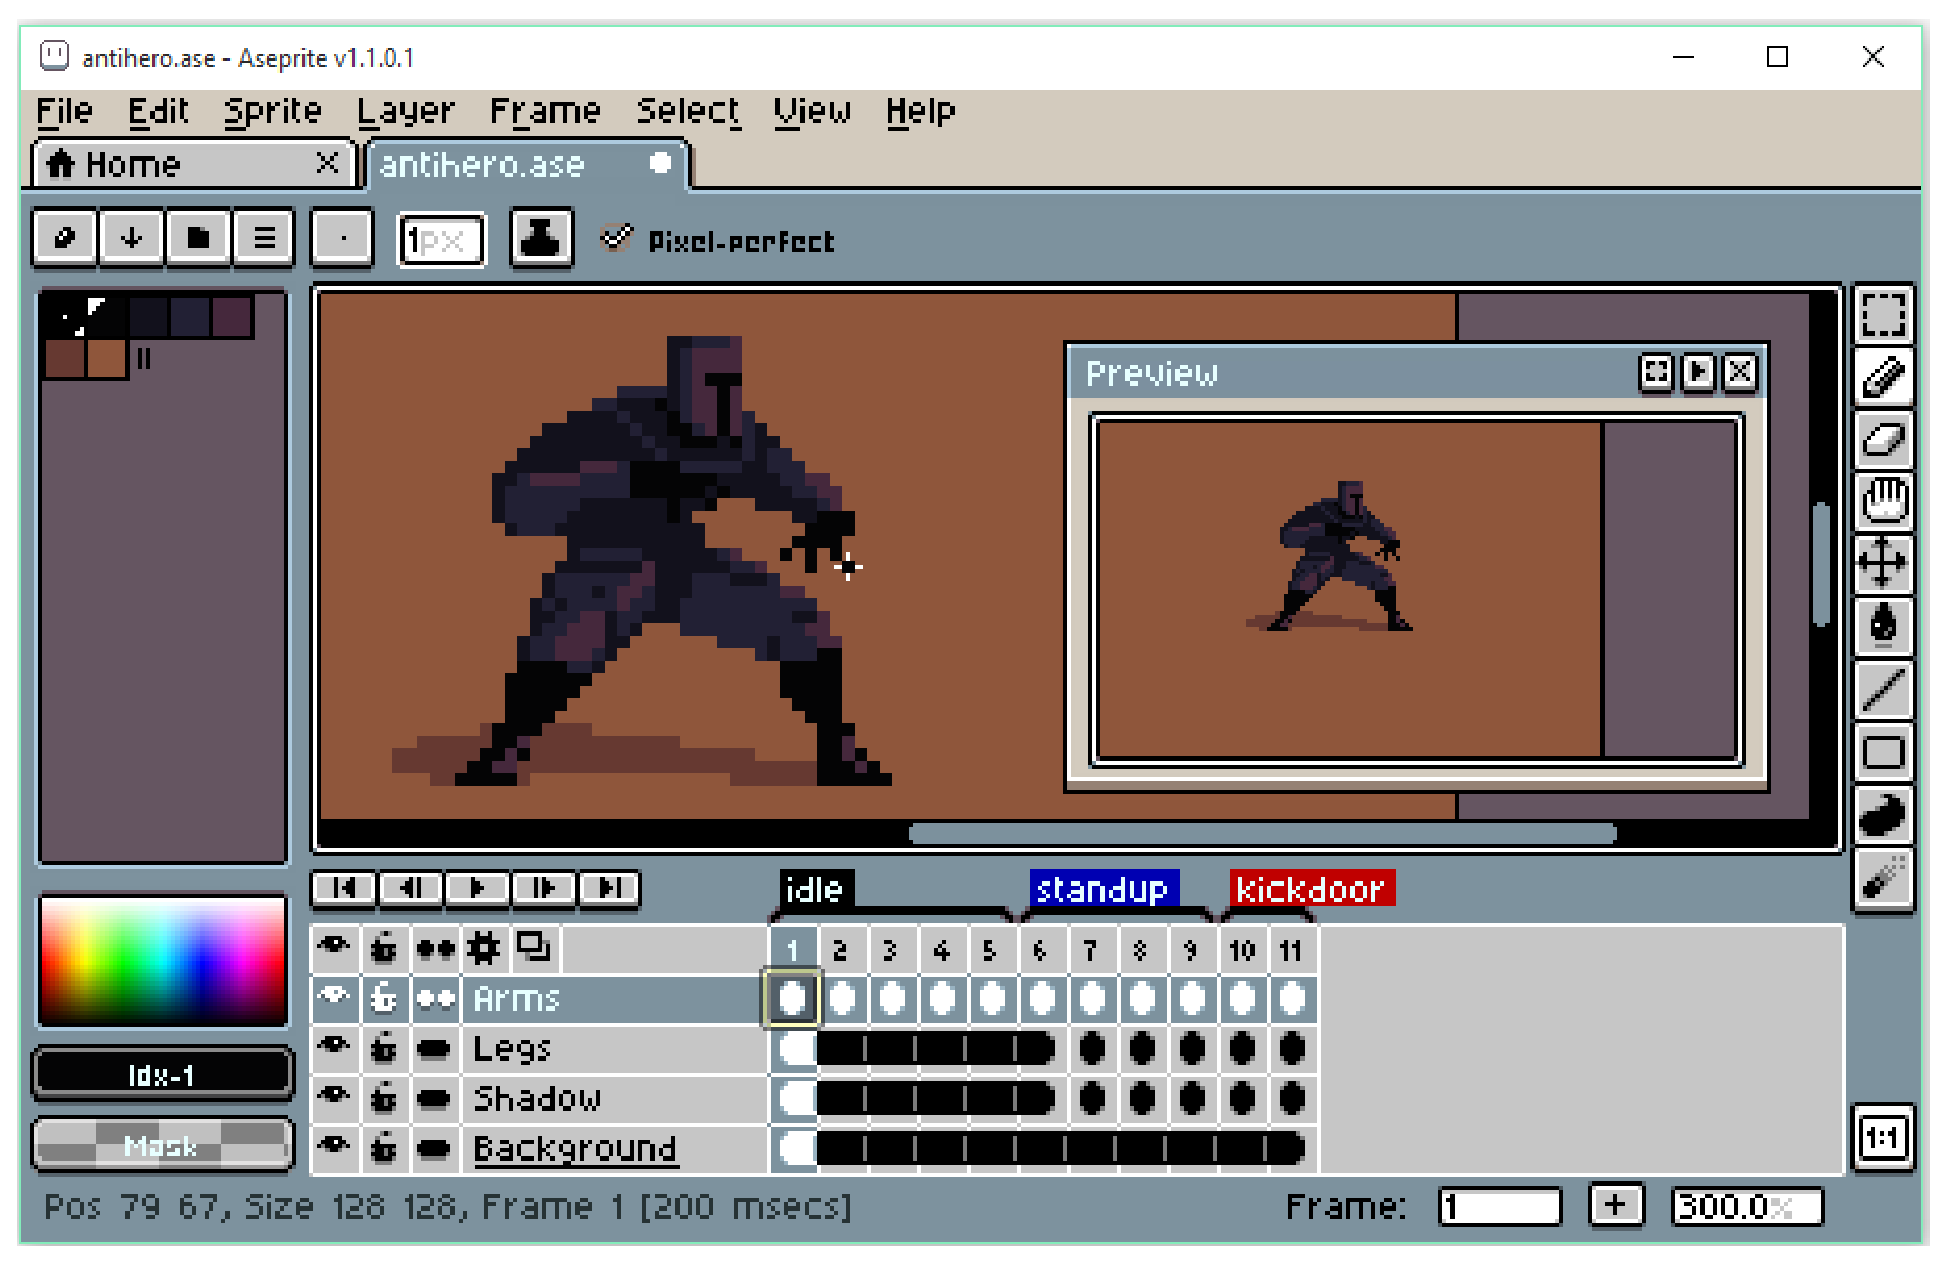
\includegraphics[scale=0.3]{figuras/aseprite.eps}
        \caption{Imagem da ferramenta Aseprite}
        \label{ferramenta_aseprite}
    \end{figure}

    \item \textbf{Pencil}
 \footnote{\url{http://www.pencil2d.org/pencil2d/}} é uma ferramenta para
 desenho e animação desenhada a mão, e utilizando desenhos em formato bitmap ou gráfico vetoriais. 
Esta ferramenta é gratuita  e open source, podendo ser encontrada em no \textit{Github}
 \footnote{\url{https://github.com/pencil2d/pencil}} ou no site da ferramenta
 \footnote{\url{http://www.pencil2d.org}}.

    \begin{figure}[h]
        \centering
            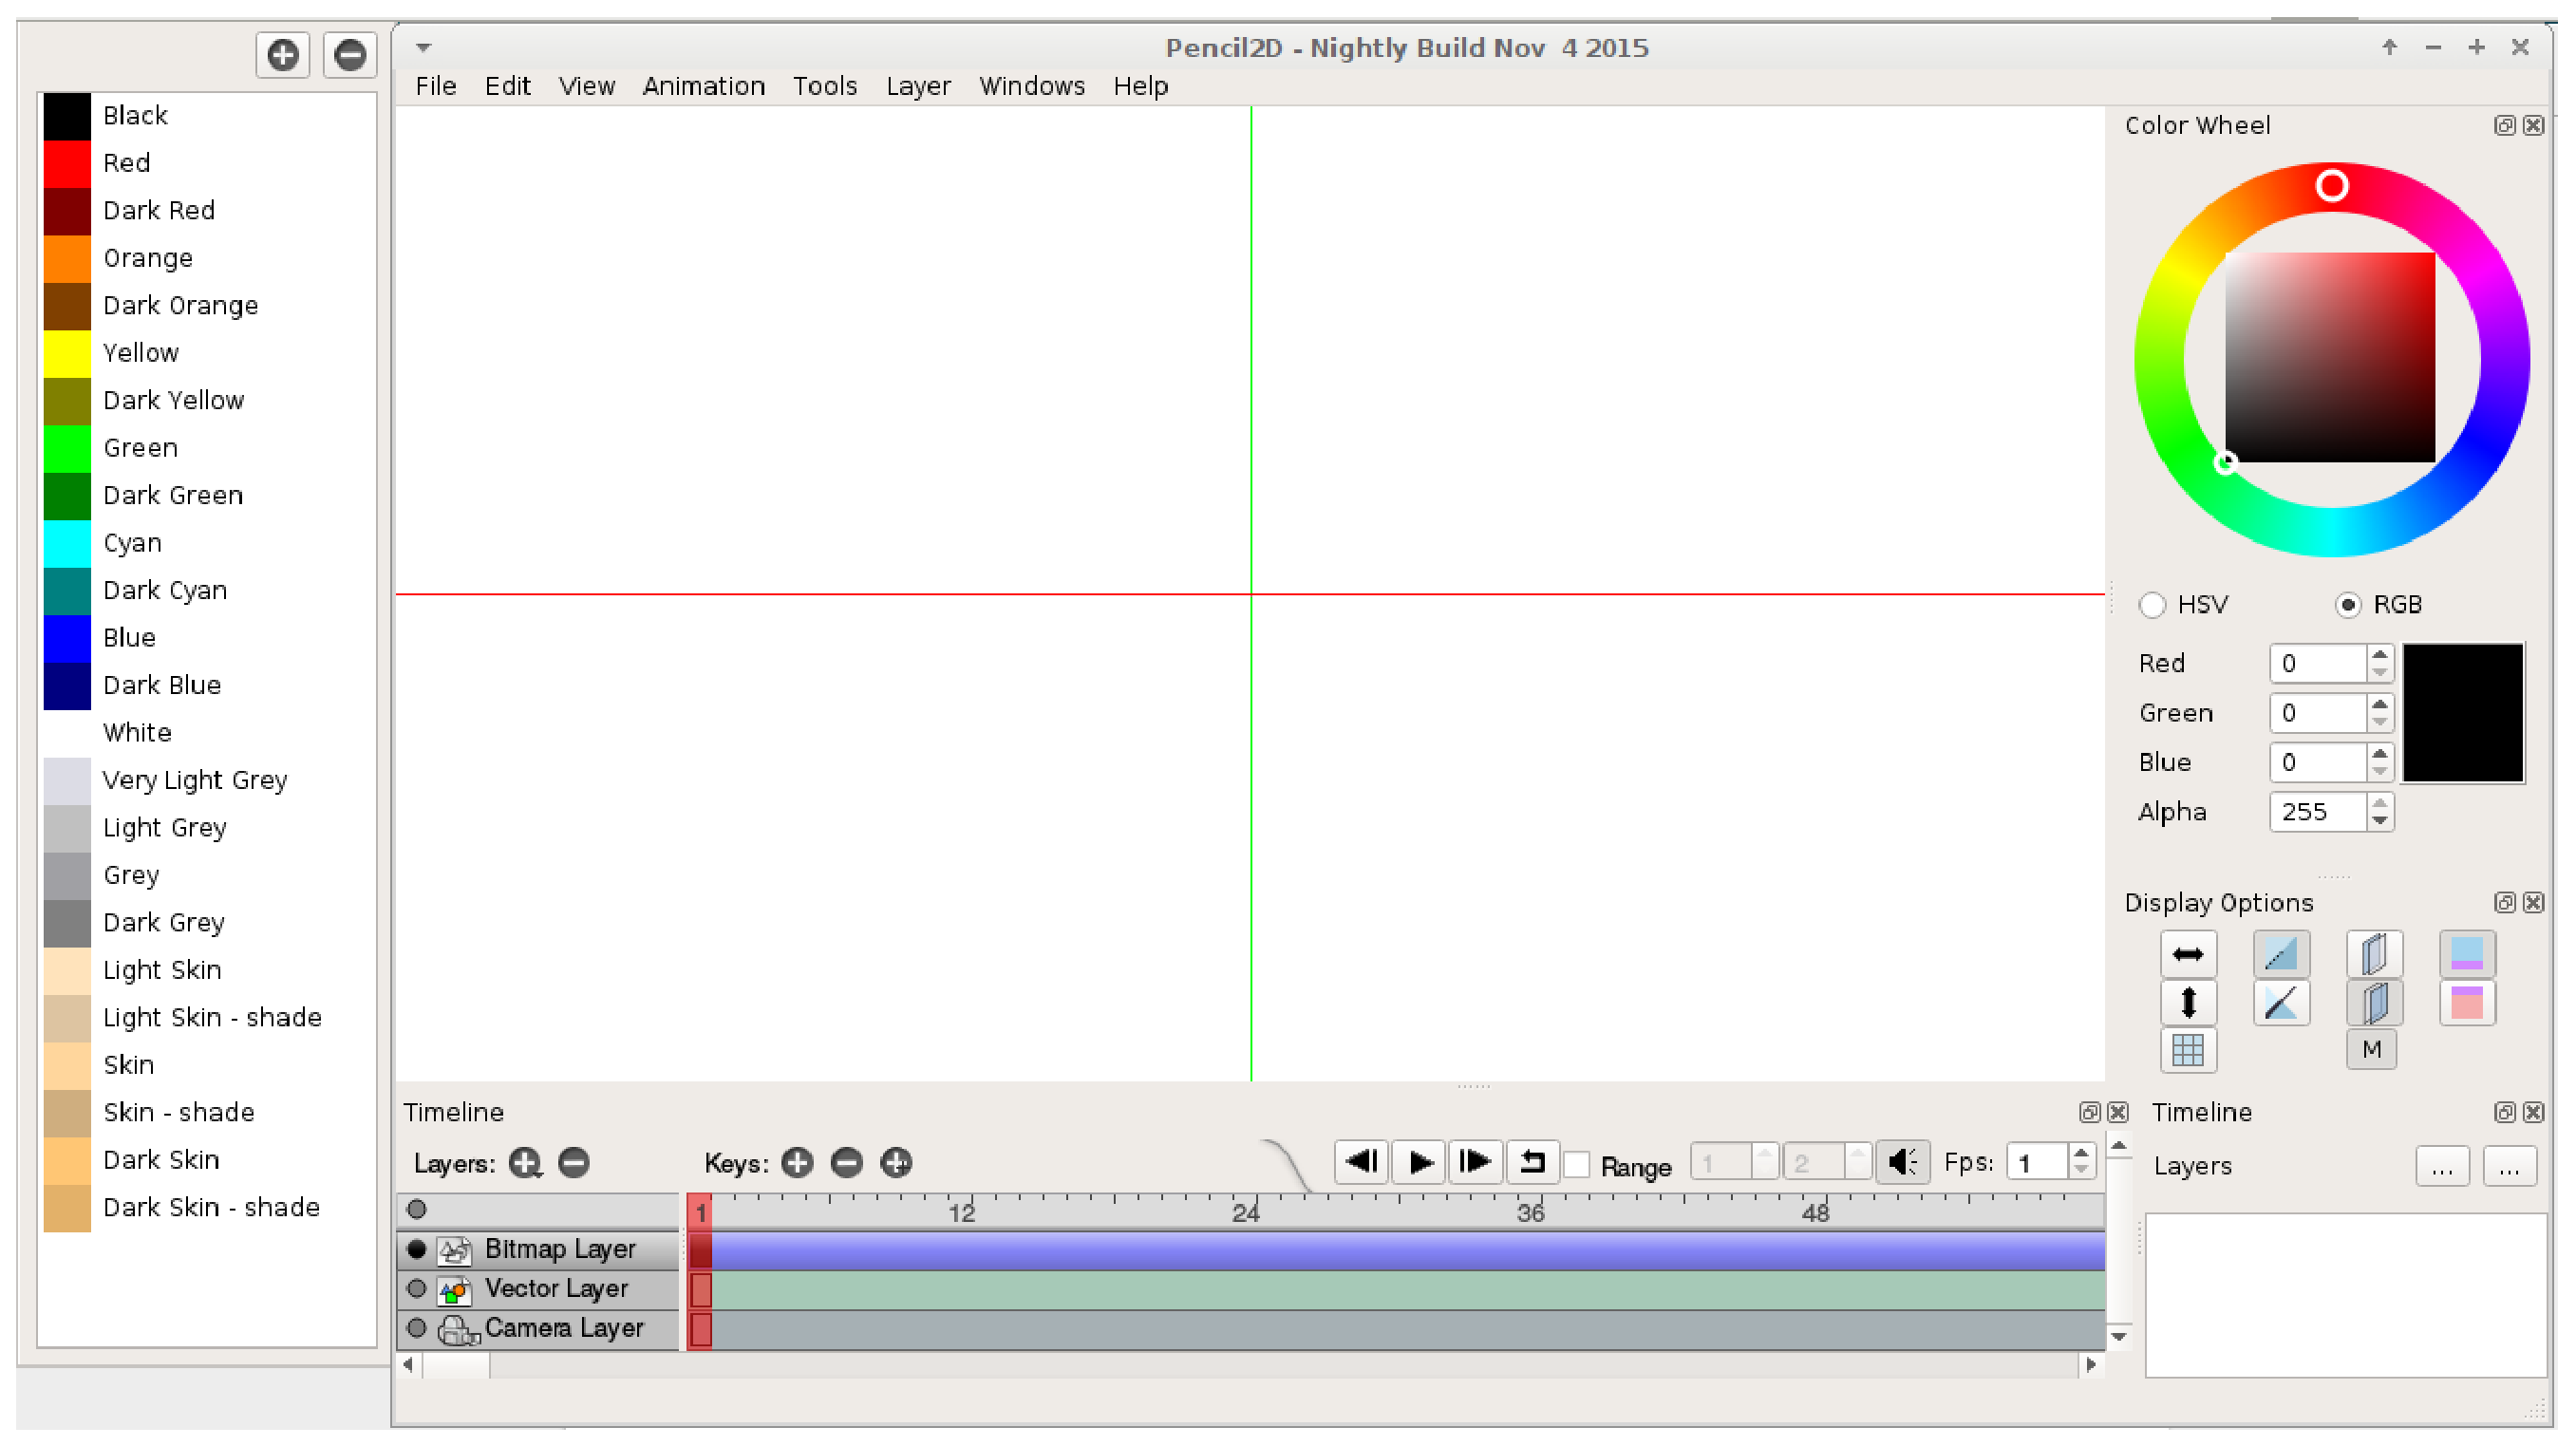
\includegraphics[scale=0.3]{figuras/pencil2D.eps}
        \caption{Imagem da ferramenta }
        \label{ferramenta_pencil2D}
    \end{figure}

    \item \textbf{Qcad}
 \footnote{\url{http://www.qcad.org/en/}} é um software para desenho
 assistido por computador em duas dimensões, permitindo a criação de desenhos técnicos como
 planos para edifícios, interiores, peças mecânicas ou esquemas e diagramas. Esta ferramenta
 e open source  e gratuita e podendo ser encontrada no \textit{Github}
 \footnote{\url{https://github.com/qcad/qcad}} ou no site da ferramenta.
 \footnote{\url{http://www.qcad.org/en/}}

    \begin{figure}[h]
        \centering
            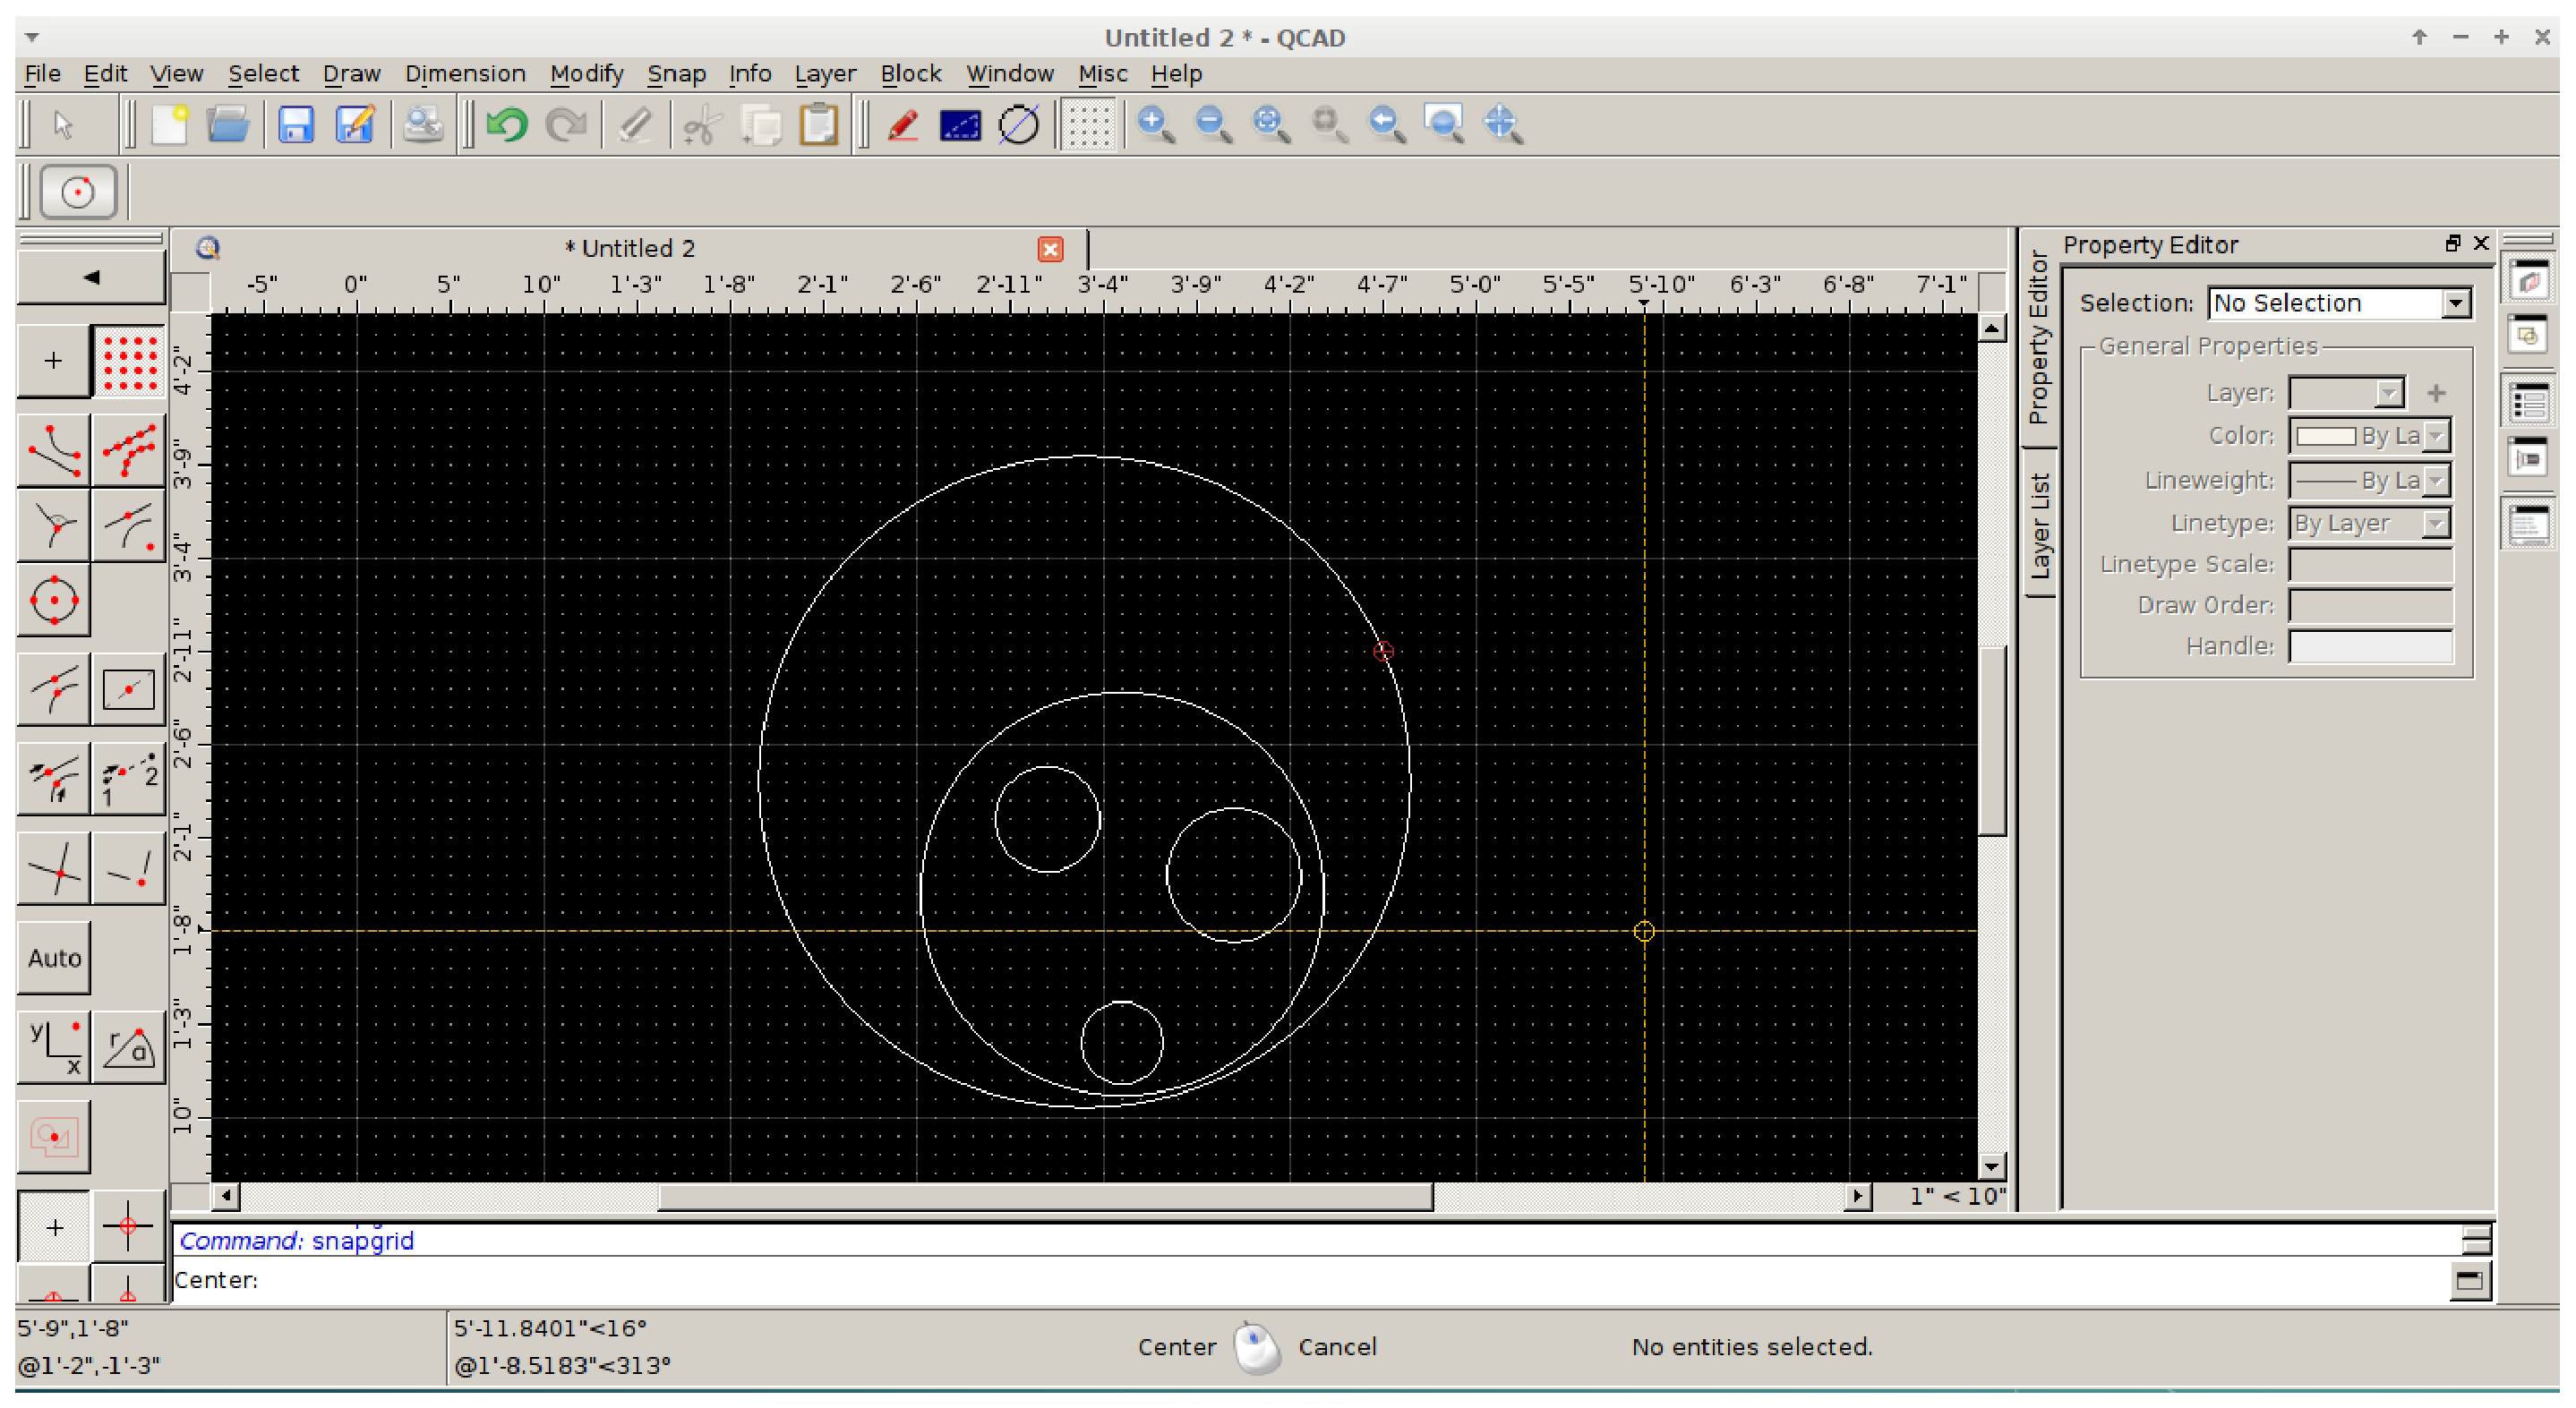
\includegraphics[scale=0.3]{figuras/qcad.eps}
        \caption{Imagem da ferramenta Qcad}
        \label{ferramenta_qcad}
    \end{figure}

    \item \textbf{Sudoku}
 \footnote{\url{https://github.com/macartur-tcc/sudoku}} é um software que foi
 desenvolvido em um curso na universidade de Hasselt na Bélgica, esta foi escrita em c++ e utilizando Qt.
 Este é um software livre e liberado para domínio publico e pode ser encontrado apenas no \textit{Github}
 \footnote{\url{https://github.com/macartur-tcc/sudoku}}.

    \begin{figure}[h]
        \centering
            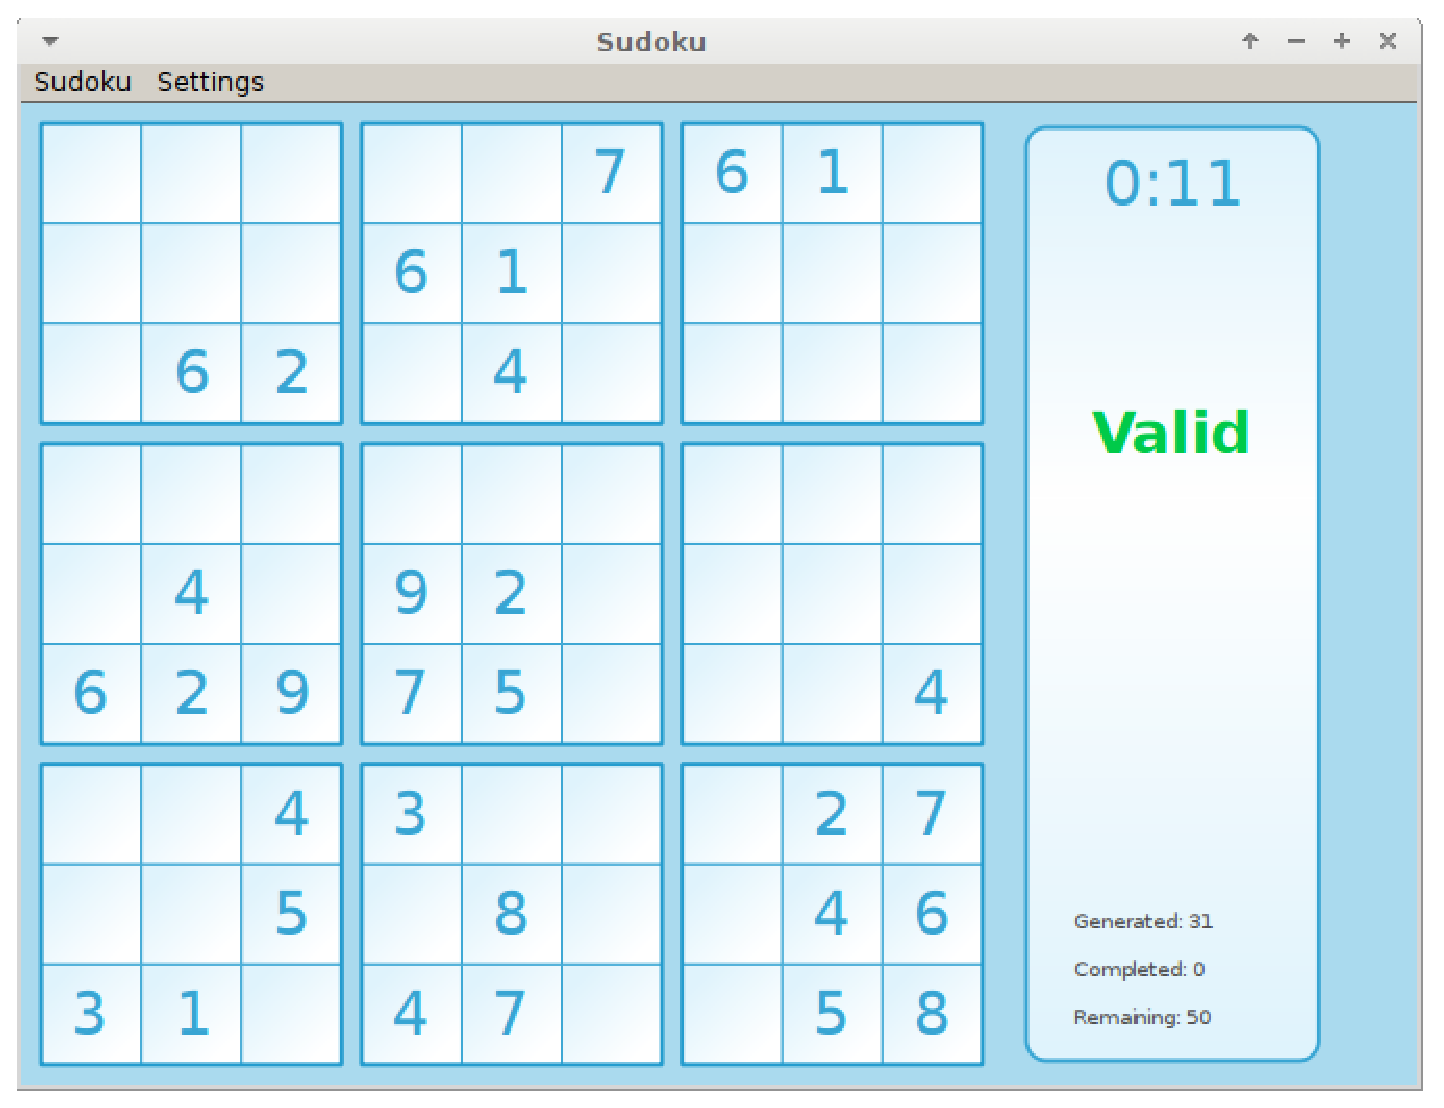
\includegraphics[scale=0.3]{figuras/sudoku.eps}
        \caption{Imagem da ferramenta Sudoku}
        \label{ferramenta_qcad}
    \end{figure}

    \item \textbf{iRecoveryplusplus}
 \footnote{\url{https://github.com/GreySyntax/iRecoveryplusplus}} é um programa projetado para
 realizar comunicação de iPod, iPhone e iPad iBoot/iBSS  com interface USB. 
Este é um software livre e sobre a licença GPV v3 e pode ser encontrado no \textit{github}
 \footnote{\url{https://github.com/GreySyntax/iRecoveryplusplus}} e é suportado em Linux, Mac OS e Windows.

\end{itemize}




\section{Ambiente}

\subsection{Ambiente Físico}

Para a realização dos estudos foi utilizado uma máquina com as
 especificações listada na tabela \ref{configuracoes_ambiente_fisico}

\begin{table}[h]
\centering
\begin{tabular}{lllll}
\textbf{Sistema Operacional} & \textit{Ubuntu} 14.04 \\ \toprule
\textbf{Kernel} & 3.19  \\ \midrule 
\textbf{Processador} & Intel i5 2.0Ghz \\ \midrule
\textbf{Memória Ram} & 4G  \\ \bottomrule 
\end{tabular} 
\caption{Configurações do Ambiente Físico}
\label{configuracoes_ambiente_fisico}
\end{table}


Nesta máquina foi instalado os programas:

\begin{itemize}
    \item \textbf{VirtualBox} (4.0) : é uma ferramenta open source sobre a
 licença GPL v2 que permite a virtualização de máquinas.
    \item \textbf{Vagrant} - (1.7.4) : ferramenta de controle de
 máquina virtual possibilitando fácil acesso, criação, destruição, ligar e 
desligar máquinas virtuals.
    \item \textbf{Git} (2.5.1) : ferramenta de controle de versão descentralizada
com o mesmo objetivo do \textit{SubVersion}(\textbf{SVN}).
\end{itemize}

\subsection{Ambiente Virtual}

\begin{itemize}

    \item \textbf{Linux}
        \subitem  O ambiente virtual Linux foi criado utilizando a box
 ubuntu/trusty64 \footnote{\url{https://atlas.hashicorp.com/ubuntu/boxes/trusty64}},
 com a configuração do Vagrantfile representada no Código \ref{vagrant_linux} e com especificações
 da máquina virtual mostradas na Tabela \ref{especificacoes_linux}.
 Depois que construída a máquina virtual foram instalados os pacotes utilizando o
 gerenciador de pacotes apt, e estão listados na Tabela \ref{pacotes_instalados_linux}.

Em ambiente Linux o compilador padrão de C++ que vem instalado é o gcc/g++, este foi
 criado pela GNU e contém um conjunto de ferramentas para realizar pré-processamento,
 compilação, montagem e link-edição. No \textit{front-end} este compilador inclui as linguagens C,
 C++, Objective-C, Fortran, Java, Ada e Go, bem como bibliotecas (stdlibc++, libgcj, entre outras).


\begin{lstlisting}[language=ruby, caption={Vagrantfile com configurações da máquina virtual linux},
                  label=vagrant_linux]
    # Vagrantfile
    Vagrant.configure(2) do |config|
        config.vm.define 'linux' do |linux|
            linux.vm.box = "ubuntu/trusty64"
            linux.vm.network 'private_network', ip: "10.10.10.4"
            linux.vm.provider "virtualbox" do |vm| 
                vm.cpus = 2
                vm.memory = 2048
            end
        end              
    end
\end{lstlisting}

\begin{table}[h]
\centering
\caption{Configurações do Ambiente Virtual Linux}
\label{especificacoes_linux}
\begin{tabular}{ll}
\textbf{Sistema Operacional} & \textit{Ubuntu} 14.04 x86\_64 \\ \toprule
\textbf{Kernel} & 3.13.0-45-generic  \\ \midrule 
\textbf{Processador} & 2 processadores Virtuais \\ \midrule
\textbf{Memória Ram} & 2GB  \\ \bottomrule 
\end{tabular} 
\end{table}

\begin{table}[h]
\centering
\caption{Pacotes instalados no Ambiente Virtual Linux}
\label{pacotes_instalados_linux}
\begin{tabular}{ll}
\textbf{Pacote} & \textbf{Versão} \\ \toprule
Qt5-default & 5.5.1 \\ \midrule 
Qt4-default & 4.8.7 \\ \midrule 
libusb-1.0-0/libusb-1.0-0-dev & 1.0.17-1ubuntu2 \\ \midrule 
libreadline6/libreadline6-dev & 6.3-4ubuntu2 amd6 \\ \midrule 
zlib1g/zlib1g-dev & 1.2.8.dfsg-1ubuntu1 amd6 \\ \midrule 
zlibc & 0.9k-4.1  \\ \midrule
g++/gcc  &  4:4.8.2-1ubuntu6 \\ \midrule 
git & 1.9.1-1 \\ \midrule 
cmake &   2.8.12.2  \\ \midrule 
ccache & 3.1.9  \\ \bottomrule 
\end{tabular} 
\end{table}

    \item \textbf{Mac OS Yosemite}
        \subitem Para o ambiente Mac OS foi utilizada uma box com o sistema
 operacional na versão Yosemite 10.10.4
 \footnote{\url{http://files.dryga.com/boxes/osx-yosemite-0.2.1.box}},
 com as configurações do Vagrantfile representada no Código \ref{vagrant_mac_os_x} e com
 especificações da máquina virtual mostradas na Tabela \ref{especificacoes_mac_os_x}.
 Após a máquina criada foi necessário instalar os pacotes utilizando o gerenciador de
 pacotes brew \footnote{\url{http://brew.sh/}}, e foram listados os pacotes listados na tabela
 \ref{pacotes_instalados_mac_os_x}.
Além dos listados foi necessário instalar o pacote " \textbf{MacOSX10.4.Universal.pkg}”
 \footnote{\url{https://github.com/macartur-tcc/aseprite/blob/master/INSTALL.md}}
 disponibilizado pela Apple  \footnote{\url{https://developer.apple.com/downloads/}}.

        \subitem Em um ambiente Mac OS o LLVM
 \footnote{LLVM: infraestrutura de compilação utilizando o principio de modularização
 e reuso, propondo otimizar a compilação, execução e link-edição de programas
 escritos em linguagens variadas} é o \textit{back-end} do compilador e como \textit{front-end}
 padrão possui o clang/clang++, que foi projetado para ser 3 vezes mais rápido
 que o gcc/g++. As linguagens aceitas pelo clang são Objective-C, Fortran,
 Ada, Haskell, Java, Python, Ruby, ActionScript, GLSL, Julia, entre outras.


\begin{lstlisting}[language=ruby, caption={Vagrantfile com configurações da máquina virtual Mac OS Yosemite},
                  label=vagrant_mac_os_x]
    # Vagrantfile
    Vagrant.configure(2) do |config|
      config.vm.define 'mac_os_x' do |mac_os_x|
        mac_os_x.vm.box = "mac_os_x"
        mac_os_x.vm.network 'private_network', ip: "10.10.10.3"
        mac_os_x.vm.synced_folder "projetos", "/vagrant", type: "rsync"

        mac_os_x.vm.provider "virtualbox" do |vm|
          vm.gui = true
          vm.memory = 2024
        end
      end
    end

\end{lstlisting}

\begin{table}[h]
\centering
\caption{Configurações do Ambiente Virtual Mac OS Yosemite}
\label{especificacoes_mac_os_x}
\begin{tabular}{ll}
\textbf{Sistema Operacional} & \textit{OS X Yosemite} x86\_64  \\ \toprule
\textbf{Kernel} & Darwin Kernel  14.4.0  \\ \midrule 
\textbf{Processador} & 2 processadores Virtuais \\ \midrule
\textbf{Memória Ram} & 2GB  \\ \bottomrule 
\end{tabular} 
\end{table}


\begin{table}[h]
\centering
\caption{Pacotes instalados no Ambiente Virtual Mac OS Yosemite}
\label{pacotes_instalados_mac_os_x}
\begin{tabular}{ll}
\textbf{Pacote} & \textbf{Versão} \\ \toprule
qt5 & 5.5.1 \\ \midrule 
qt4 & 4.8.7 \\ \midrule 
libusb & 1.0.20 \\ \midrule 
readline & 6.3-8 \\ \midrule
zlib & 1.2.8 \\ \midrule
git & 1.9.1-1 \\ \midrule
cmake & 3.3.0  \\ \midrule
binutils & 2.25-4 \\ \midrule
ccache & 3.2.3 \\ \bottomrule
\end{tabular} 
\end{table}

    \item \textbf{Windows}
        \subitem Para o ambiente virtual Windows foi utilizado uma box com
 o sistema operacional Windows7 \footnote{\url{https://vagrantcloud.com/datacastle/boxes/windows7}},
 com as configurações do Vagrantfile mostradas no Código \ref{vagrant_windows},
 e com especificações da máquina virtual mostradas na Tabela \ref{especificacoes_windows}.
 Para a utilização de um ambiente de desenvolvimento no windows é necessário a instalação
 do software \textit{cygwin} \footnote{\url{https://www.cygwin.com/}}, que permite a instalação
o dos pacotes necessários para a criação do ambiente igual ao Unix.
 Utilizando o \textit{cygwin} é necessário instalar todos os pacotes para o sistema 
conseguir compilar programas em C/C++, para isto foram instalados os programas 
que estão listadas na tabela \ref{pacotes_instalados_windows}.

\begin{lstlisting}[language=ruby, caption={Vagrantfile com configurações da máquina virtual Windows 7},
                  label=vagrant_windows]
    #Vagrantfile
    Vagrant.configure(2) do |config|
      config.vm.define 'win7' do |win|
        win.vm.box = 'win7ie8'
        win.vm.network 'private_network', ip: '10.10.10.5'
        win.vm.provider 'virtualbox' do |vm|
              vm.cpus = 2
              vm.gui = true
              vm.memory = 1024
        end
      end
    end
\end{lstlisting}

\begin{table}[h]
\centering
\caption{Configurações do Ambiente Virtual Windows 7}
\label{especificacoes_windows}
\begin{tabular}{ll}
\textbf{Sistema Operacional} & \textit{Windows 7} x86\\ \toprule
\textbf{Kernel} & CYGWIN\_NT-6.1  \\ \midrule 
\textbf{Processador} & 2 processadores Virtuais \\ \midrule
\textbf{Memória Ram} & 2GB  \\ \bottomrule 
\end{tabular} 
\end{table}


\begin{table}[h]
\centering
\caption{Pacotes instalados no Ambiente Virtual Windows 7}
\label{pacotes_instalados_windows}
\begin{tabular}{ll}
\textbf{Pacote} & \textbf{Versão} \\ \toprule
qt5-devel-tools  &  \\ 
qt5-translations & 5.5.1-1  \\ 
todos os pacotes que começam com este nome libQt5 & \\ \midrule

qt4-designer-plugin-webkit  & \\
qt4-devel-tools & 4.8.7-1 \\ 
qt4-qtconfig & \\ \midrule

libusb1.0 & 1.0.19-1 \\ \midrule


libreadline-devel & 6.3.8-1 \\ \midrule

zlib & 1.2.8 \\ \midrule
git & 2.5.3-1 \\ \midrule
ccache & 3.1.9-2 \\ \midrule
cmake & 3.3.2-1 \\ \midrule
cygwin-devel & 2.2.1 \\ \midrule
cygwin64-gcc-core & 4.9.2-1 \\ \midrule
gcc-core & \\ \midrule
gcc/g++ & 4.9.3-1 \\ 
make & 4.1-1 \\ \bottomrule
\end{tabular} 
\end{table}
\end{itemize}

\section{Restrições de Compilação}

\subsection{Restrição Global}

    A utilização do linker gold não permite a compilação em todos os ambientes,
 pois é aplicada apenas a sistemas de arquivos binários ELF e nos ambientes
 Windows e Mac OS Yosemite os sistemas de arquivos são PE ou PE32+ e PEF, respectivamente.

\subsection{Restrição Especifica}
    Um ambiente \textit{mingw} ou \textit{cygwin} não possui suporte
 a biblioteca glibc \footnote{\url{https://www.gnu.org/software/gnulib/manual/html\_node/execinfo\_002eh.html}},
 o que fez com que o projeto Qcad, que necessita do header exec\_info.h não podesse ser compilado.

    Para alguns projetos foi necessário realizar modificações para a compilação
 dos mesmos nos diferentes sistemas operacionais. Estas alterações foram colocadas
 na branch master do repositório modificado, utilizando um \textit{fork} do Github
  \footnote{\url{https://github.com/macartur-tcc/}} que contém todos os projetos.
 Esta restrição não impediu a compilação dos projetos nos diferentes ambientes.

\section {Estudo de Caso}

\subsection{Aplicado no Ambiente}

Os casos de guardas de inclusão foram realizados utilizando \textit{script} de \textit{benchmark},
 na qual os métodos detalhados na Seção \ref{include_guards_section} foram
 aplicados a 10 mil arquivos com uma pequena quantidade de Código
 \ref{codigo_27} e incluidos 3 vezes ao arquivo \textbf{main.cpp} utilizando
 \ref{codigo_28}. Cada um destes foram aplicados aos diferentes ambientes de
 desenvolvimento.

\begin{lstlisting}[language=C++,caption={Template de arquivo .hpp utilizado no \textit{benchmark}},
                                                   label=codigo_27]

  // <NUMERO>.hpp

  const int int<NUMERO> = <NUMERO>;

\end{lstlisting}

\begin{lstlisting}[language=C++,caption={Template de arquivo main.cpp utilizado no \textit{benchmark}},
                                                          label=codigo_28]

    // main.cpp

    /* headers a serem incluidos   */

    ...

    int main(){return 0;}
\end{lstlisting}

Os scripts abordam os métodos:

\begin{itemize}
	\item guarda de Inclusão Externa;
	\item guarda de Inclusão Interna;
	\item \textit{pragma once};
	\item guarda de Inclusão Interna primeiro que \textit{pragma once};
	\item \textit{pragma once} primeiro que  Guarda de Inclusão Interna;
	\item guarda de Inclusão Externa + \textit{pragma once};
	\item redundância de Guarda de Inclusão.
\end{itemize}

\subsection{Aplicado no Projeto}

Antes da realização do estudo de caso foi necessário identificar quais
 as técnicas que poderiam ser aplicadas em cada um dos projetos.
 As tabelas \ref{tecnicas_que_podem_ser_aplicadas_codigo}, \ref{tecnicas_que_podem_ser_aplicadas_flag} e 
\ref{tecnicas_que_podem_ser_aplicadas_ferramenta} mostram esta analise.


\begin{table}[h]
\centering
\caption{Técnicas que podem ser aplicadas ao código}
\label{tecnicas_que_podem_ser_aplicadas_codigo}
\begin{tabular}{llll}
\textbf{Projeto} & \textbf{pragma once} & \textbf{Forward Declaration} & \textbf{Pimpl Idiom}  \\ \toprule 
iRecoveryplusplus & SIM & SIM & SIM  \\ 
Sudoku &  SIM & SIM & SIM  \\ 
Pencil & SIM & NÃO &  SIM \\ 
Aseprite &  SIM & NÃO & NÃO  \\ 
Qcad &  SIM & NÃO & NÃO  \\ \bottomrule
\end{tabular} 
\end{table}

\begin{table}[h]
\centering
\caption{\textit{Flags} que podem ser utilizadas}
\label{tecnicas_que_podem_ser_aplicadas_flag}
\begin{tabular}{lll}
\textbf{Projeto} & \textbf{Makafile} &  \textbf{Otimização de Baixo Nível} \\ \toprule
iRecoveryplusplus & SIM & SIM\\ 
Sudoku &  SIM & SIM  \\ 
Pencil &  SIM & SIM  \\ 
Aseprite & SIM & SIM  \\ 
Qcad &   SIM & SIM\\ \bottomrule
\end{tabular} 
\end{table}

\begin{table}[h]
\centering
\caption{Ferramentas que podem ser utilizadas}
\label{tecnicas_que_podem_ser_aplicadas_ferramenta}
\begin{tabular}{lll}
\textbf{Projeto} &  \textbf{Ccache} & \textbf{Gold} \\ \toprule 
iRecoveryplusplus &  SIM & SIM \\ 
Sudoku            &  SIM & SIM \\ 
Pencil            &  SIM & SIM \\ 
Aseprite          &  SIM & SIM \\ 
Qcad              &  SIM & SIM \\ \bottomrule
\end{tabular} 
\end{table}


\subsubsection{Alteração de Código}

 Para as alterações de código, cada caso foi criado
 uma branch com suas modificações e estas estão no repositório
 destinado ao TCC\footnote{\url{https://github.com/macartur-tcc/}}.

    \begin{enumerate}
        \item Pragma Once
        \subitem Neste estudo de caso os arquivos de header foram alterados
 com a inclusão da diretiva “\#pragma once” no inicio de cada arquivo.
 No projeto aseprite está sendo removida a diretiva, pois todos os arquivos já possuem.
Estas alterações estão na branch “\textit{pragma\_once}” dos projetos que foi possível aplicar.
        \item Forward Declaration
        \subitem Neste estudo de caso os headers foram alterados para reduzir
 a quantidade de headers de todos os cabeçalhos e das implementação.
 Para isso foram removidos headers redundantes e que referenciava
 ponteiros e referências de endereço.
Estas alterações estão na branch "\textit{forward\_declaration}" dos projetos que foi possível aplicar.
        \item Técnicas de Pimpl Idiom
        \subitem Neste estudo de caso atributos e métodos privados foram removidos do cabeçalho
 e incluídos nos arquivos de implementação, como no exemplo de código \ref{exemplo_implementacao_pimpl}
 da seção \ref{Pimpl_Idiom}
 que demostra como aplicar a técnica.
Estas alterações estão na branch "\textit{pimpl}" dos projetos que foi possível aplicar.
    \end{enumerate}

\subsubsection{Alteração de flags de Compilação}

        \begin{enumerate}
            \item makefile
                \subitem Neste estudo de casos no momento da utilização do makefile
 será utilizado as flags: -j2,-j4,-j6,-j8 e -j10. Com este resultará na relação entre
a compilação e a quantidade de \textit{jobs}(\textit{threads}).
            \item Otimização de Baixo Nível
                \subitem Neste estudo de caso todos os arquivos Makefile serão
 alterados para receber a flags: -O, -O0, -O2, -Ofast, -O3, -Os,-Og.
 Com estes resultados será possível verificar a relação do tempo gasto com
 o tempo de otimização do compilador.
        \end{enumerate}

\subsubsection{Ferramentas Auxiliares}

        \begin{enumerate}
               \item CCache
                    \subitem Neste estudo de caso em cada projeto será adicionado
 a palavra ccache antes de cada linha de compilação. Será utilizado as
 configurações padrão do ccache, e antes de cada compilação para ter certeza
 que toda a cache será removida utilizará o comando ccache -C e ccache -c.
                \item Gold
                    \subitem Neste estudo de caso será ativado o ld.gold
 utilizando a flag:-Wl,-fuse-ld=gold como mostrado na seção \ref{Gold}. Assim  a
 compilação irá deixar de utilizar o linker padrão e utilizará o linker
 otimizado para sistema ELF.
        \end{enumerate}

\subsubsection{Passos de Compilação dos projetos}

\begin{itemize}
       \item {iRecoveryplusplus}
        \subitem Para compilar o projeto iRecoveryplusplus é necessário
 realizar o clone do projeto no github, e compilar utilizando os comandos no Código 
\ref{clonando_irecoveryplusplus}.


\begin{lstlisting}[language=bash, caption={Clonado e compilando o projeto iRecoveryplusplus},
                  label=clonando_irecoveryplusplus]

    # clonando o projeto
    $ git clone https://github.com/macartur-tcc/iRecoveryplusplus.git 
    $ cd iRecoveryplusplus

    # compilando no Linux, Mac OS Yosemite ou Windows 7
    $ make linux 
    
    # compilar utilizando o linker gold no Linux
    $ make linux  CC="gcc -Wl,-fuse-ld=gold" CXX="g++ -Wl,-fuse-ld=gold"

    # compilar utilizando a ferramenta ccache
    $ make linux CC="ccache gcc" CXX="ccache g++"

    # removendo arquivos binarios gerados
    rm bin/*
\end{lstlisting}

    \item \textbf{Sudoku}
    \subitem Para compilar o projeto Sudoku é necessário realizar o clone do projeto
no github utilizando os comandos no Cógido \ref{clonando_sudoku}.
\footnote{Neste projeto e necessário remover a flag -archi386 do arquivo Makefile gerado na raiz, pois em sistemas Mac OS esta flag causa erro.}

\begin{lstlisting}[language=bash, caption={Clonado e compilando o Projeto Sudoku},
                  label=clonando_sudoku]

    # clonando projeto do github 
    $ git clone https://github.com/macartur-tcc/sudoku.git 
    $ cd sudoku/src

    # gerando makefile
    $ qmake Sudoku_release.pro

    # compilando no Linux, Mac OS ou Windows 7
    $ make

    # compilar no Linux utiizando o linker gold
    $ make  CC="gcc -Wl,-fuse-ld=gold" CXX="g++ -Wl,-fuse-ld=gold"

    # compilando utilizando a ferramenta ccache
    $ make CC="ccache gcc" CXX="ccache g++"

    # remover arquivos binarios gerados
    $ make clean
    
\end{lstlisting}

    \item \textbf{Pencil}
    \subitem Para compilar o projeto Pencil é necessário realizar
 o clone do projeto no github e executar os comandos mostrados no
 Código \ref{clonando_pencil} 

\begin{lstlisting}[language=bash, caption={Clonado Projeto Pencil},
                  label=clonando_pencil]
    #clonando o projeto do github
    $ git clone https://github.com/macartur-tcc/pencil.git
    $ cd pencil

    # gerando makefile para ambiente Linux e Windows 7
    $ qmake -r

    # gerando makefile para ambiente Mac OS Yosemite
    $ qmake -r RESOURCES=./pencil.qrc  
    
    # compilando 
    $ make

    # compilando utilizando a ferramenta ccache
    $ make CC="ccache gcc" CXX="ccache g++"

    # compilando utilizando gold
    make CC="gcc -Wl,-fuse-ld=gold" CXX="g++ -Wl,-fuse-ld=gold"

    # removendo arquivos binarios gerados
    $ make clean

\end{lstlisting}

    \item \textbf{Aseprite}
    \subitem Para compilar o projeto Aseprite é necessário fazer o clone do projeto,
 gerar os arquivos makefile seguindo os comandos no Código \ref{clonando_aseprite}.

\begin{lstlisting}[language=bash, caption={Clonado Projeto Aseprite e criando diretório de Compilação},
                  label=clonando_aseprite]
    # clonado projeto do github
    $ git clone https://github.com/macartur-tcc/aseprite.git
    $ cd aseprite

    # criando diretorio para compilar o projeto
    $ mkdir build
    $ cd build

    # gerando makefile do projeto no Linux e Windows 7
    $ cmake -G .. "Unix Makefiles"

    # gerando makefile no Mac OS Yosemite
    $ cmake -G ... "Unix Makefiles" -DCMAKE_OSX_ARCHITECTURES:STRING=i386  -DCMAKE_OSX_DEPLOYMENT_TARGET:STRING=10.4  -DCMAKE_OSX_SYSROOT:STRING=/SDKs/MacOSX10.4u.sdk
    
    # compilando o projeto com ccache no Linux Windows 7
    $ cmake -G .. "Unix Makefiles"  -DCMAKE_CXX_COMPILER="ccache"  -DCMAKE_CXX_COMPILER_ARG1="g++" -DCMAKE_C_COMPILER="ccache" -DCMAKE_C_COMPILER_ARG1="gcc"

    # compilando projeto com ccache no Mac OS Yosemite
    $ cmake -G .. "Unix Makefiles"  -DCMAKE_CXX_COMPILER="ccache"  -DCMAKE_CXX_COMPILER_ARG1="g++" -DCMAKE_C_COMPILER="ccache" -DCMAKE_C_COMPILER_ARG1="gcc"  -DCMAKE_OSX_ARCHITECTURES:STRING=i386  -DCMAKE_OSX_DEPLOYMENT_TARGET:STRING=10.4  -DCMAKE_OSX_SYSROOT:STRING=/SDKs/MacOSX10.4u.sdk

    # compilando com o linker gold no Linux
    $ CC="gcc  -Wl,-fuse-ld=gold" CXX="g++ -Wl,-fuse-ld=gold" cmake .. -G "Unix Makefiles"

    # removendo arquivos binarios
    $ make clean

\end{lstlisting}


    \item \textbf{Qcad}
    \subitem Para compilar o projeto Qcad é necessário clonar o
 projeto no github, gerar os arquivos makefile e compilar
 utilizando os comandos descritos no Código \ref{clonando_qcad}.

\begin{lstlisting}[language=bash, caption={Clonado Projeto Qcad},
                  label=clonando_qcad]

    #clonando projeto do github
    $ git clone https://github.com/macartur-tcc/qcad.git
    $ cd qcad

    # compilando no Linux e Windows 7
    $ qmake -r
    
    # compilando no Mac OS Yosemite
    qmake -spec macx-g++ -r

    # compilando no Linux, Windows7 e Mac OS Yosemite
    $ make

    # compilando com a ferramenta ccache
    $ make CC="ccache gcc" CXX="ccache g++"

    # compilando com o linker gold
    $ make  CC="gcc -Wl,-fuse-ld=gold" CXX="g++ -Wl,-fuse-ld=gold"

    # removendo arquivos binarios gerados
    $ make clean

\end{lstlisting}
\end{itemize}


\section{Montagem de Scripts}


Os scripts foram elaborados utilizando a linguagem de programação python,
 e estão sendo armazenados no github
\footnote{\url{https://github.com/macartur-tcc/tcc_scripts}}.


\subsection{Aplicado ao Ambiente}\label{Amplicação ao Ambiente}

Para o estudo aplicado ao ambiente foi criado um script de benchmark utilizando
 a linguagem python, e foi detalhado no apêndice na seção Benchmark \ref{script_bench_mark}.

A Tabela \ref{tab:modelo_guards} representa o modelo utilizado na coleta dos dados,
 contendo Guarda de Inclusão Externa(GIE), Guarda de Inclusão Interna(GII),
 Pragma Once(PO), Guarda de Inclusão Interna Primeiro que Pragma Once(GIIPPO),
 Pragma Once Primeiro que Guarda de Inclusão Interna (POPGII),
 Guarda de Inclusão Externa e Pragma Once (GIEPPO) e
 Redundância de Guarda de Inclusão(RGI).

\begin{table}[!ht]
\centering
\caption{Template de amostra de Guardas de Inclusão}
\label{tab:modelo_guards}
\begin{tiny}
\begin{tabular}{lp{1cm}p{1cm}p{1cm}p{1cm}p{1cm}p{1cm}p{1cm}p{1cm}}

\textbf{Tipo} & \multicolumn{7}{l}{Utilização de Guarda de Inclusão} \\
\textbf{Medida} & \multicolumn{7}{l}{Tempos em segundos } \\
\textbf{Amostras} & \textbf{GIE} & \textbf{GII} & \textbf{PO} & 
\textbf{GIIPPO} & \textbf{POPGII} & \textbf{GIEPPO} & \textbf{RGI} \\ \toprule
 1  &  &  &   &   &   &   &  \\ 
 2  &  &  &   &   &   &   &  \\ 
 3  &  &  &   &   &   &   &  \\ 
 4  &  &  &   &   &   &   &  \\ 
 5  &  &  &   &   &   &   &  \\ 
 6  &  &  &   &   &   &   &  \\ 
 7  &  &  &   &   &   &   &  \\ 
 8  &  &  &   &   &   &   &  \\ 
 9  &  &  &   &   &   &   &  \\ 
 10 &  &  &   &   &   &   &  \\ \bottomrule
 Média: & & & & &   &   &    \\ 
\end{tabular}
\end{tiny}
\end{table}


\subsection{Aplicado a Projeto}

Para realizar as compilações dos projetos foi criado um script de recompilação que
 segue no código \ref{script_recompilacoes}, com este é possível alterar entre
 branch para compilar as alterações de código dos projetos,
 executar comandos antes e depois de cada compilação.
 Para receber todos estes comandos foi necessário a leitura de um arquivo de
 configuração de cada projeto contendo a localização do projeto,
 localização do makefile, comandos que serão executados antes e depois
 da compilação.
 Este arquivo foi escrito em yaml e seguindo o template do código
 \ref{template_para_script_recompilacoes}.
Para a contagem do tempo de compilação foi utilizado o módulo datetime do python,
 realizando a diferença do tempo inicial e final do tempo de compilação.

Após a execução do script será preenchida as tabelas abaixo, e gerado gráficos para melhor
analisar os resultados. 


\begin{table}[!ht]
\centering
\tiny
\caption{Modelo Alteração de Código}
\label{tab:modelo_alteracao_de_codigo}
\begin{tabular}{lllll}
\textbf{<Nome do Projeto>} & \textbf{master} & \textbf{pragma once} & \textbf{forward declaration} & \textbf{private implementation}   \\ \toprule
1                             &      &     &     &        \\ 
2                             &      &     &     &        \\ 
3                             &      &     &     &        \\ 
4                             &      &     &     &        \\ 
5                             &      &     &     &        \\ 
6                             &      &     &     &        \\ 
7                             &      &     &     &        \\ 
8                             &      &     &     &        \\ 
9                             &      &     &     &        \\ 
10                            &      &     &     &        \\ \bottomrule
Média                         &      &     &     &        \\ 
\end{tabular}
\end{table}


\begin{table}[!ht]
\centering
\tiny
\caption{Modelo Flags de Otimização da Compilação}
\label{tab:modelo_otimizacao_compilacao}
\begin{tabular}{llllllll}
\textbf{<Nome do Projeto>} & \textbf{-O} & \textbf{-O0} & \textbf{-O2} & \textbf{-O3} & \textbf{-Os} & \textbf{-Ofast} & \textbf{-Og} \\ \toprule
1                          &             &              &              &              &              &                 &        \\ 
2                          &             &              &              &              &              &                 &        \\ 
3                          &             &              &              &              &              &                 &        \\ 
4                          &             &              &              &              &              &                 &        \\ 
5                          &             &              &              &              &              &                 &        \\ 
6                          &             &              &              &              &              &                 &        \\ 
7                          &             &              &              &              &              &                 &        \\ 
8                          &             &              &              &              &              &                 &        \\ 
9                          &             &              &              &              &              &                 &        \\ 
10                         &             &              &              &              &              &                 &        \\ \bottomrule
Média                      &             &              &              &              &              &                 &        \\ 
\end{tabular}
\end{table}

\begin{table}[!ht]
\centering
\tiny
\caption{Modelo Flags de Processamento Paralelo}
\label{tab:modelo_flag_processamento_paralelo}
\begin{tabular}{llllll}
\textbf{<Nome do Projeto>} & \textbf{-j 2} & \textbf{-j 4} & \textbf{-j 6} & \textbf{-j 8} & \textbf{-j10}  \\ \toprule
1                                    &    &     &     &     &        \\ 
2                                    &    &     &     &     &        \\ 
3                                    &    &     &     &     &        \\ 
4                                    &    &     &     &     &        \\ 
5                                    &    &     &     &     &        \\ 
6                                    &    &     &     &     &        \\ 
7                                    &    &     &     &     &        \\ 
8                                    &    &     &     &     &        \\ 
9                                    &    &     &     &     &        \\ 
10                                   &    &     &     &     &        \\ \bottomrule
Média                                &    &     &     &     &        \\ 
\end{tabular}
\end{table}

\begin{table}[!ht]
\centering
\tiny
\caption{Modelo Ferramentas Auxiliares}
\label{tab:modelo_ferramentas_auxliares}
\begin{tabular}{lll}
\textbf{<Nome do Projeto>} & \textbf{gold} & \textbf{ccache}   \\ \toprule
1                                    &     &        \\ 
2                                    &     &        \\ 
3                                    &     &        \\ 
4                                    &     &        \\ 
5                                    &     &        \\ 
6                                    &     &        \\ 
7                                    &     &        \\ 
8                                    &     &        \\ 
9                                    &     &        \\ 
10                                   &     &        \\ \bottomrule
Média                                &     &        \\ 
\end{tabular}
\end{table}
